
\subsection{Tercer sprint de producción}
Esta etapa contiene el desarrollo del nivel tres del juego. El panorama general abarca un nivel de manera ascendente en un terreno rocoso. Después se llega al jefe que tiene forma de jaguar Tepeyóllotl.

Primero se empieza con el maquetado del nivel, para establecer el tamaño del nivel, pues esta vez será de manera vertical el diseño, y la cámara solo se moverá en esa dirección. Se establece también donde debe ir cada objeto o enemigo junto con anotaciones necesarias para la comprensión posterior, como son direcciones de movimiento o acciones que deben realizarse. Aquí se debe tomar muy en cuenta el tamaño del personaje a jugar si no, no se podrá avanzar en el nivel ya que se da la situación a atorarse debido al tamaño, incluido el espacio para saltar. Lo anterior se puede ver en la figura \ref{fig:n01}.
\begin{figure}[htbp]
	\centering
	\subfigure[Primera parte del nivel]{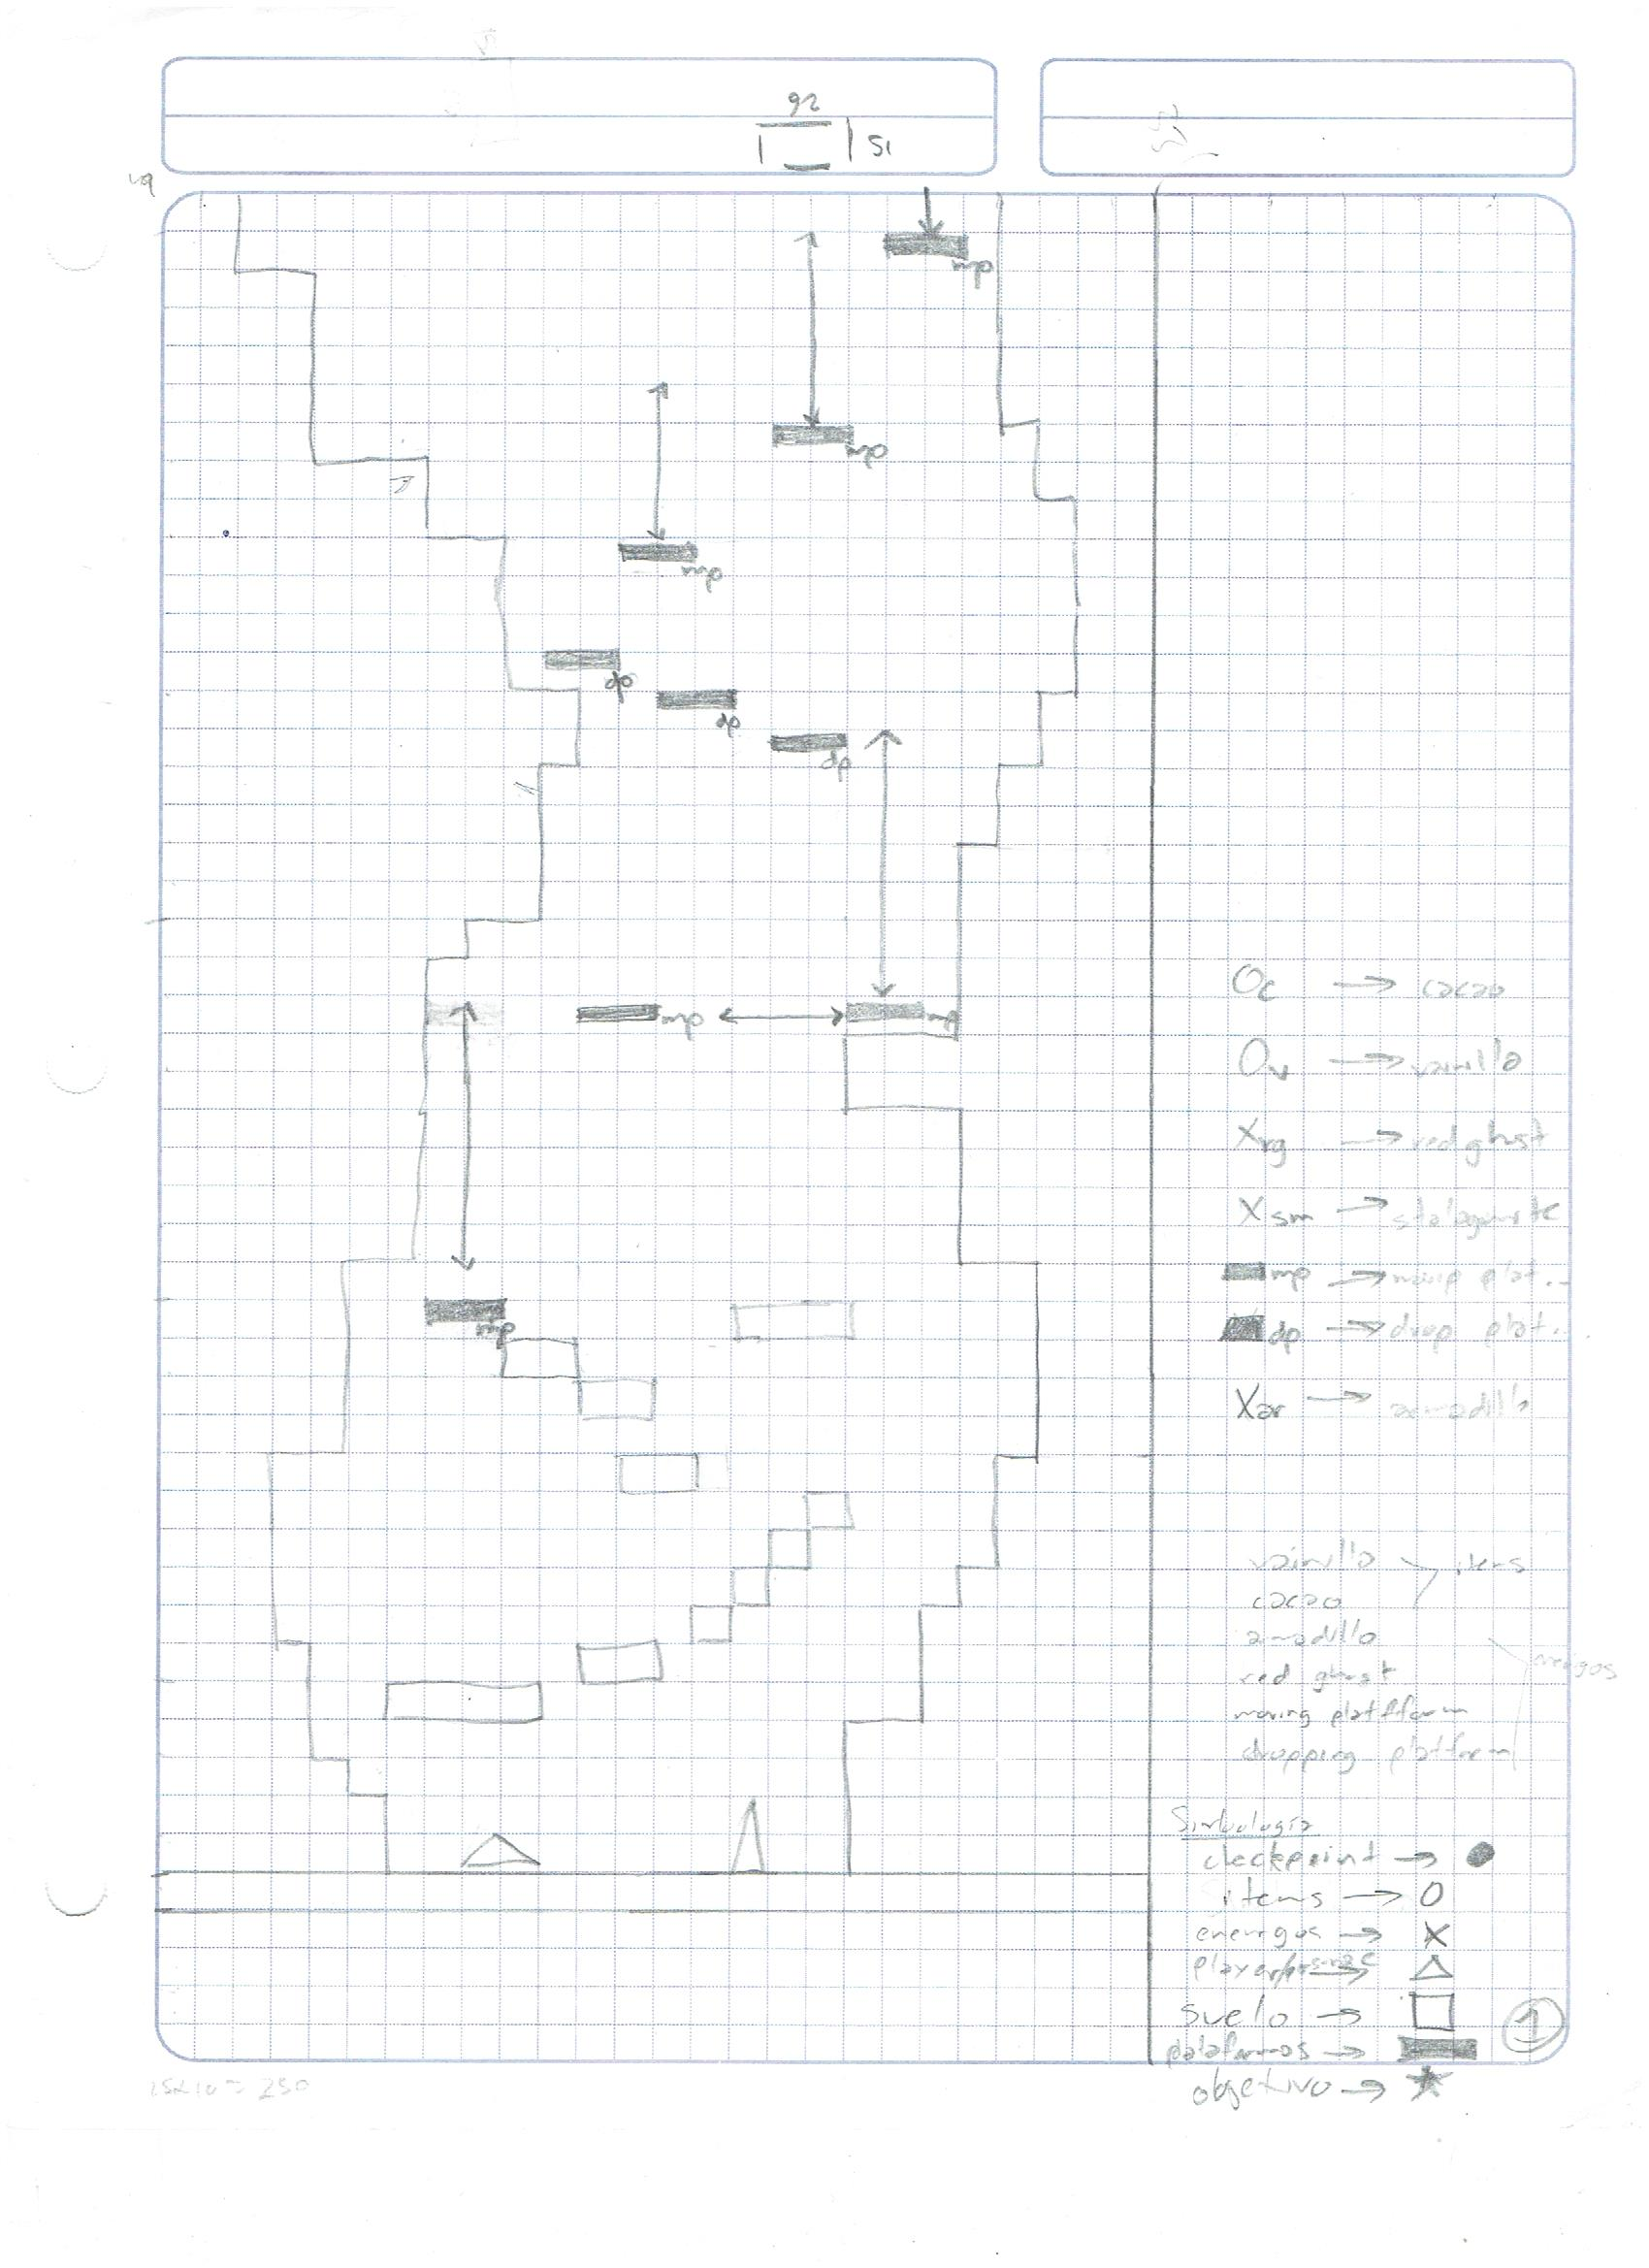
\includegraphics[width=5cm]{03TrabajoRealizado/DocProduccionR/imagenes/n3/01.jpeg}}
	\subfigure[Segunda parte del nivel]{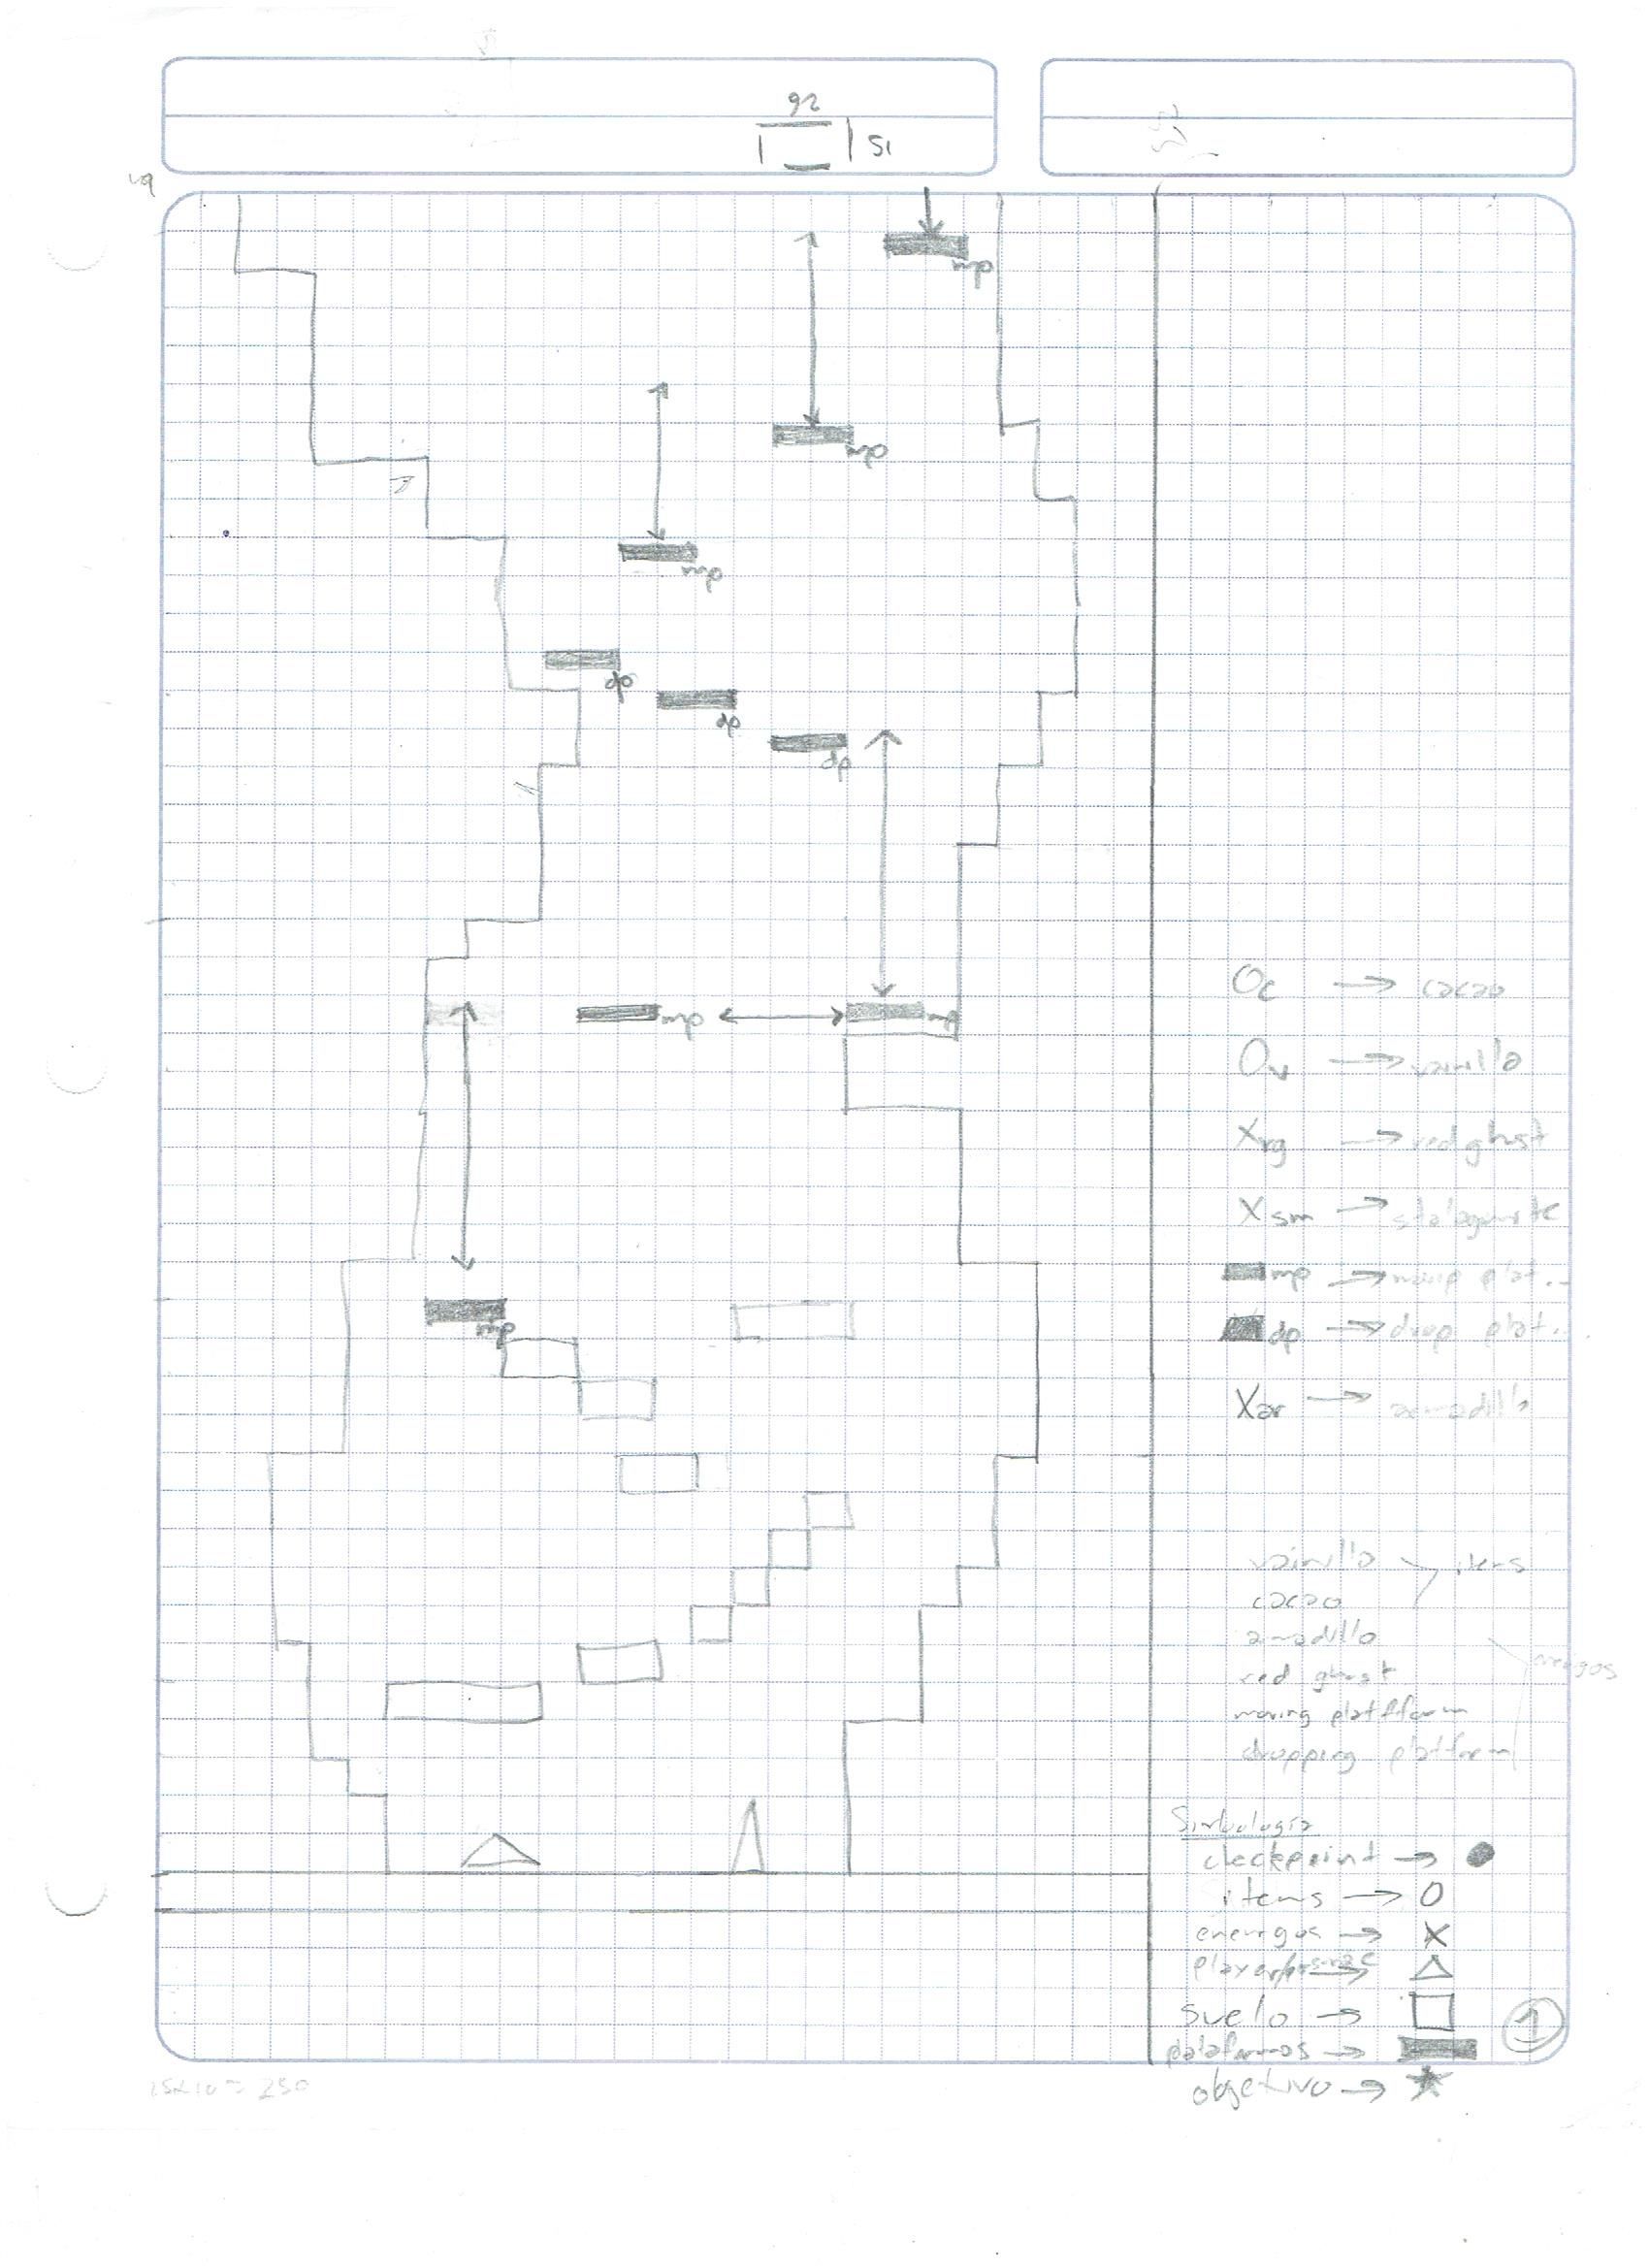
\includegraphics[width=5cm]{03TrabajoRealizado/DocProduccionR/imagenes/n3/02.jpeg}}
	\subfigure[Tercera parte del nivel]{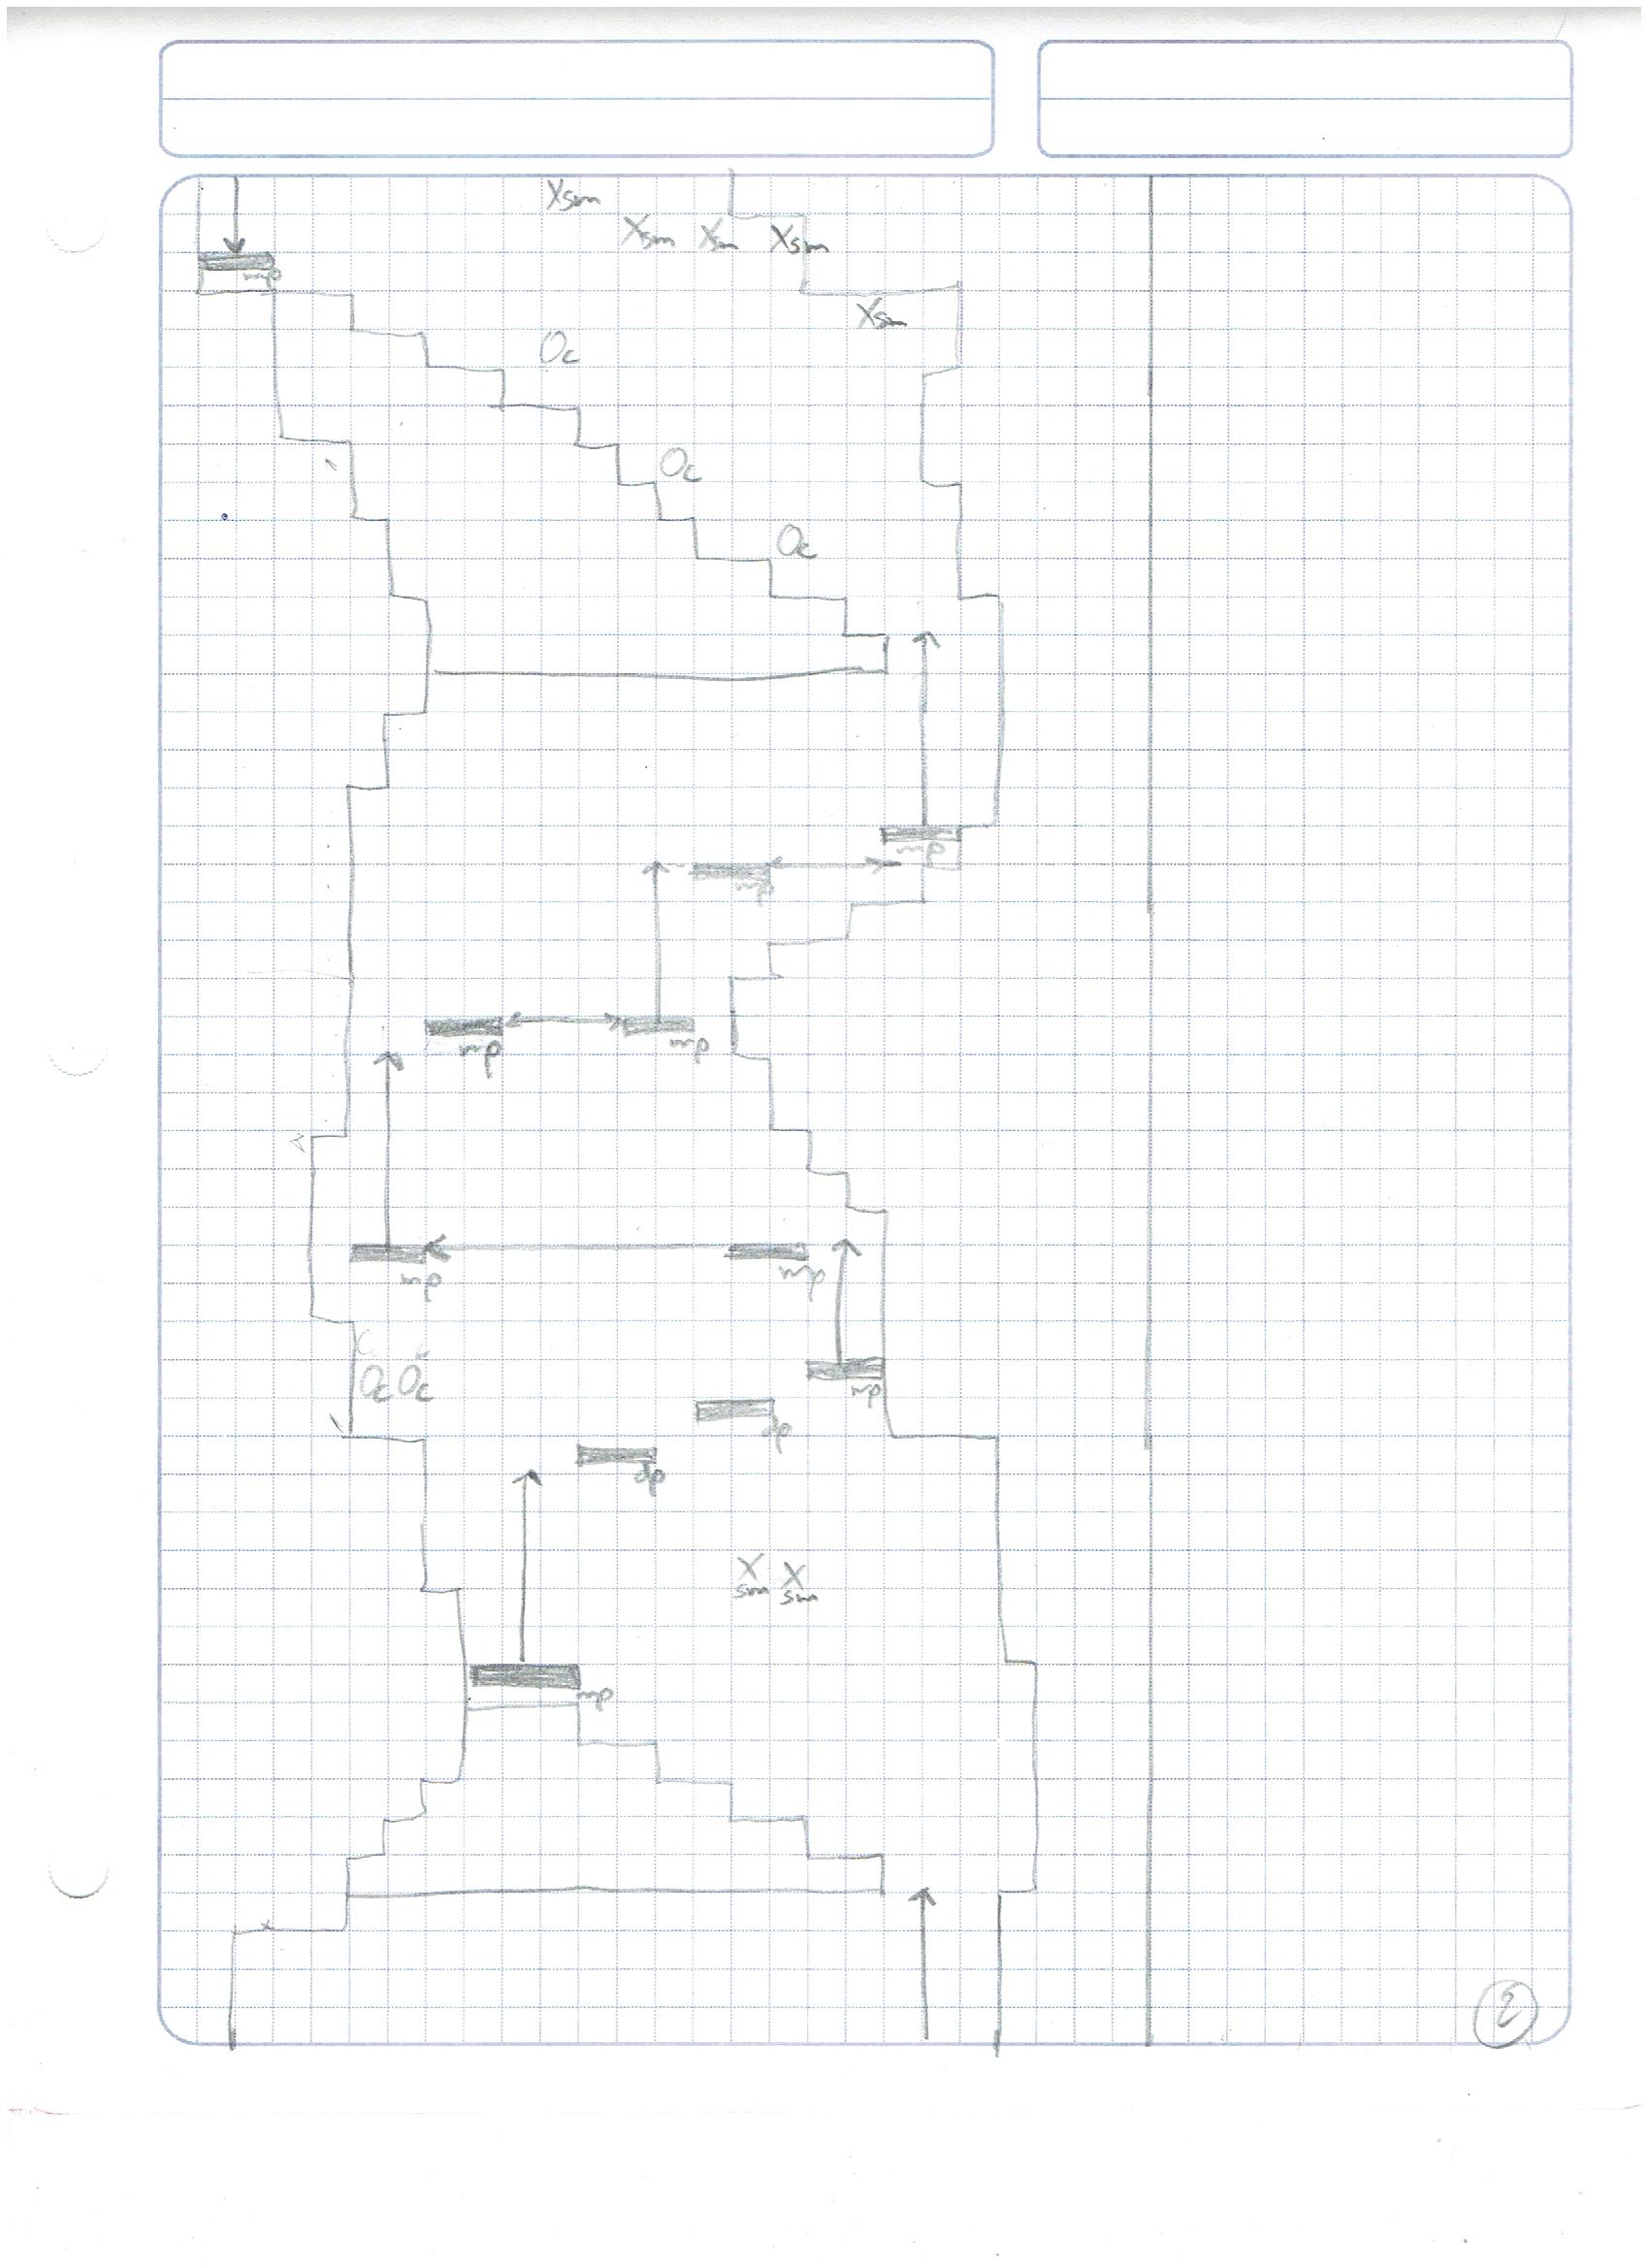
\includegraphics[width=5cm]{03TrabajoRealizado/DocProduccionR/imagenes/n3/03.jpeg}}
	\subfigure[Cuarta parte del nivel]{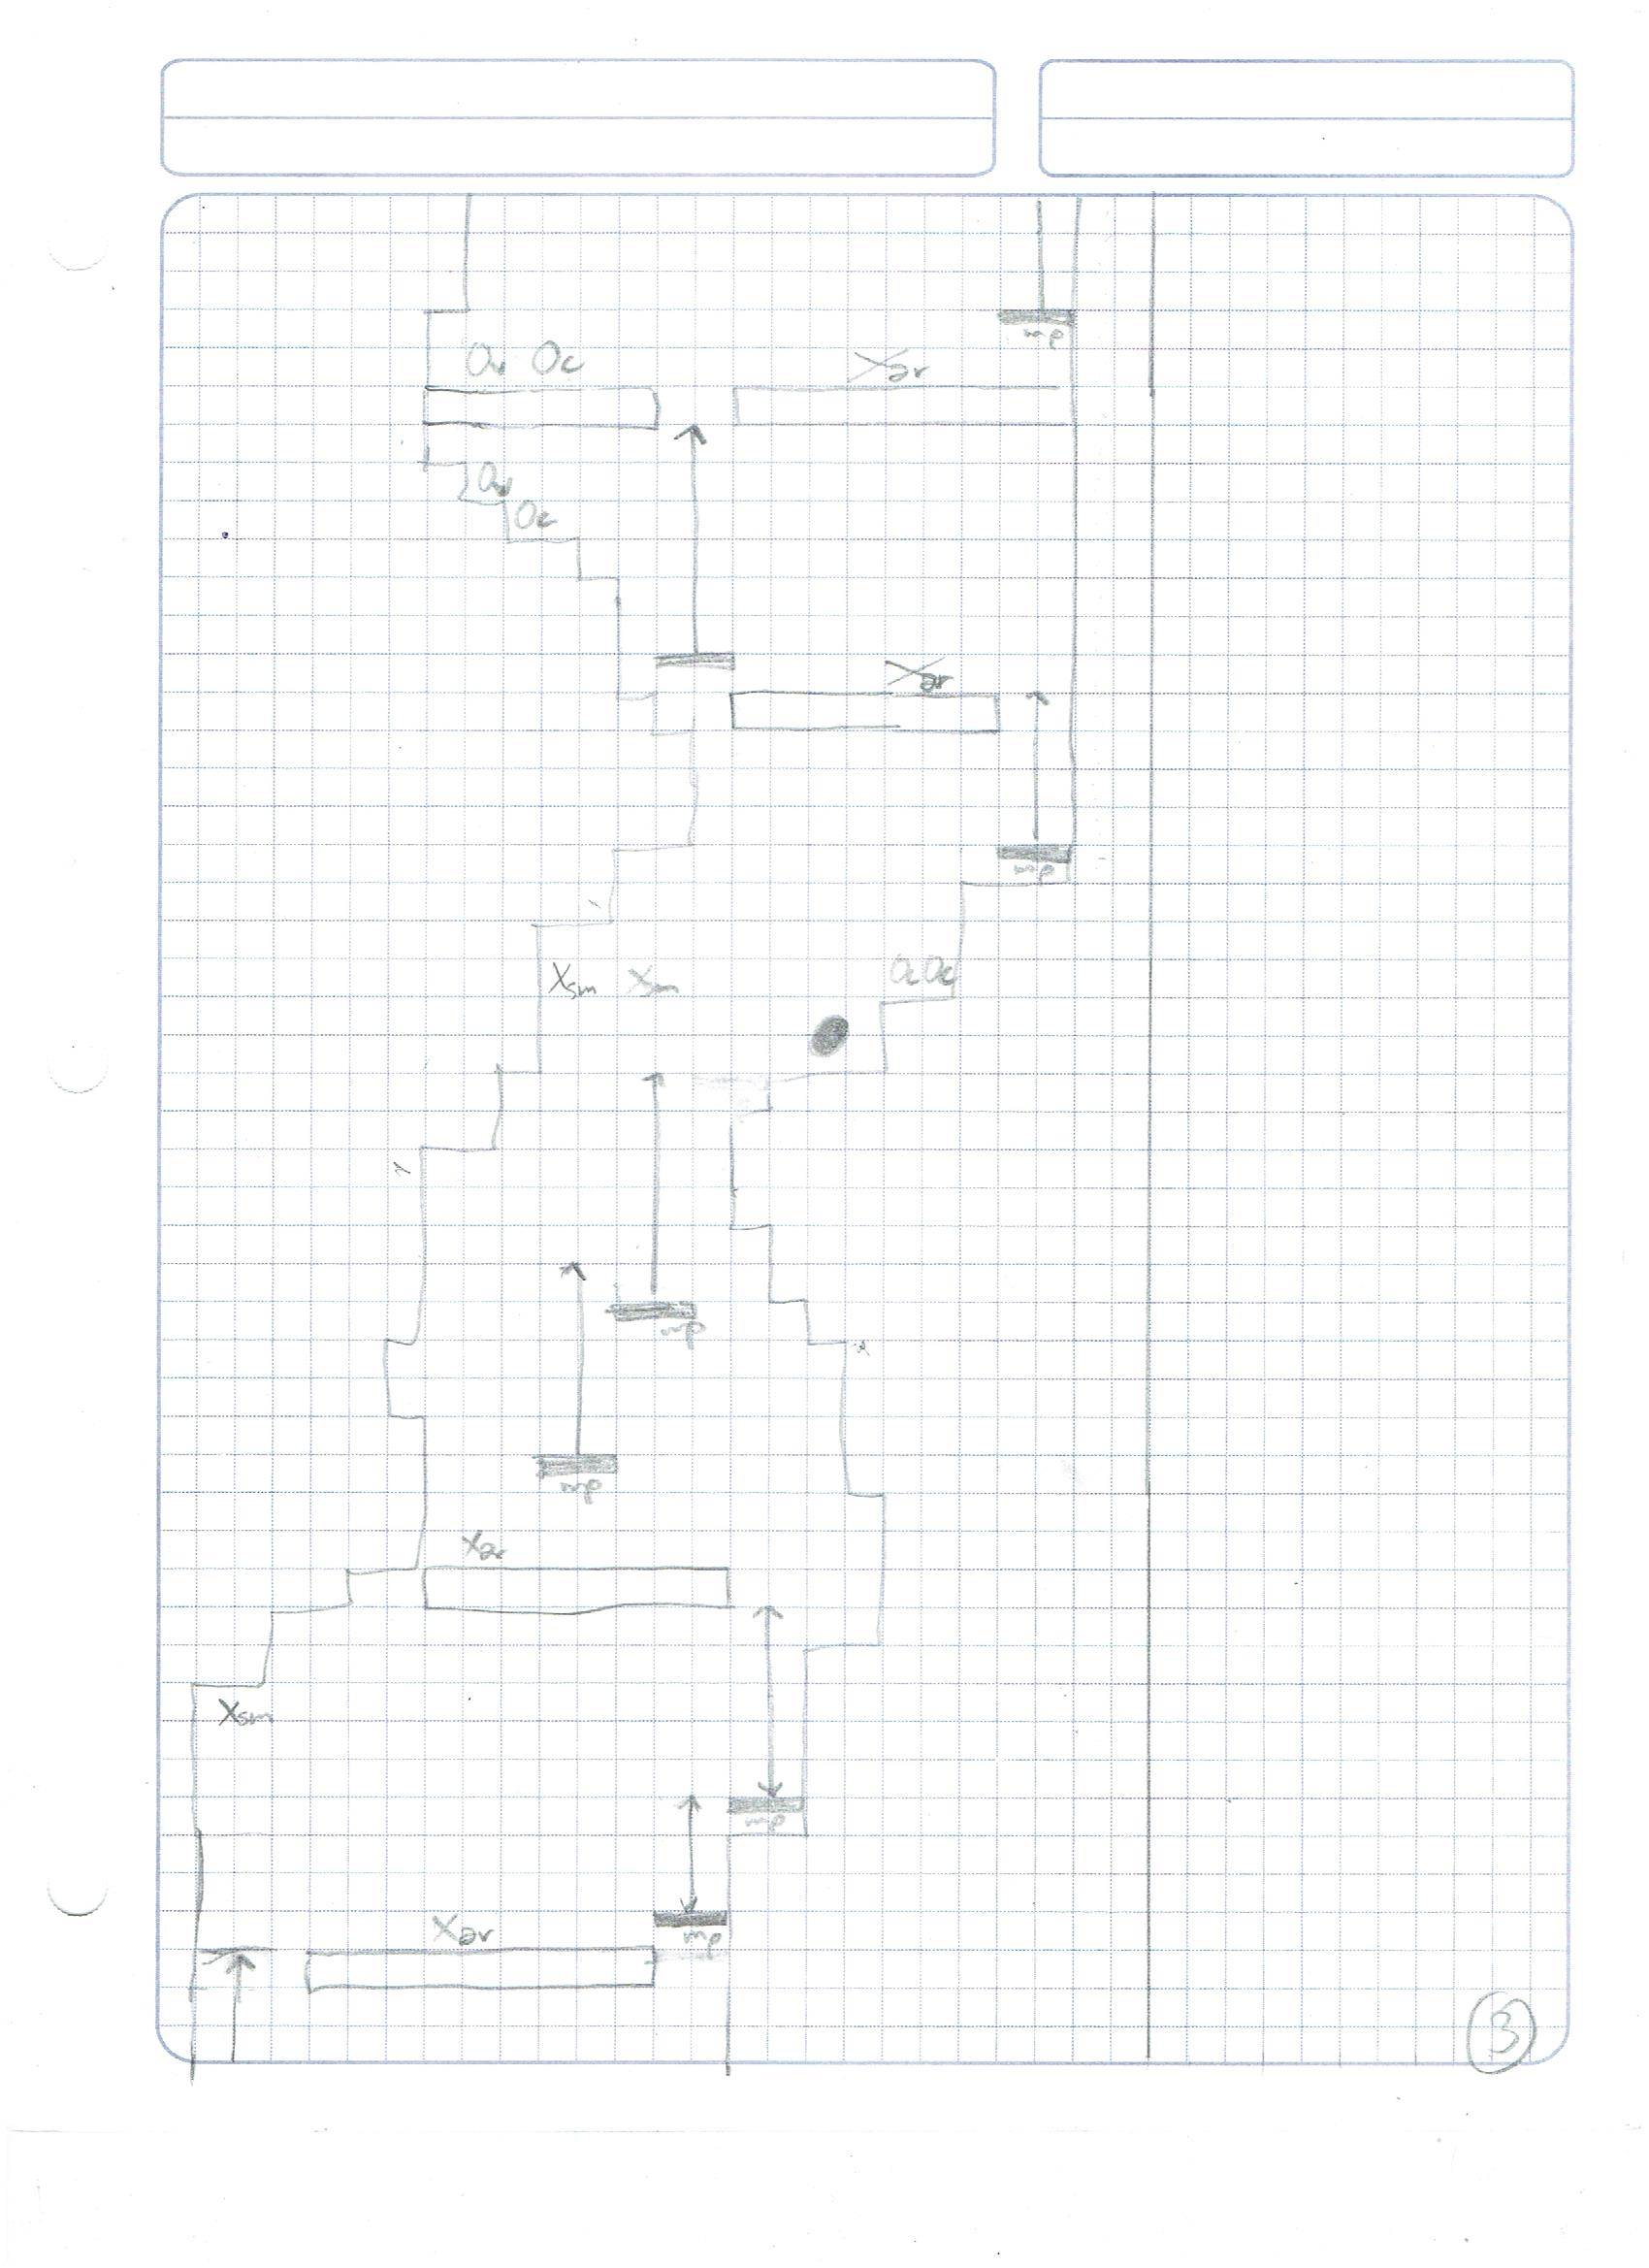
\includegraphics[width=5cm]{03TrabajoRealizado/DocProduccionR/imagenes/n3/04.jpeg}}
	\caption{Maquetado de nivel tres} \label{fig:n01}
\end{figure}  

Después se lleva la tarea de tomar todos los componentes solo de manera visual y adecuar el tamaño necesario, tomando en cuenta las medidas de los componentes anteriores. Dichas imágenes se pueden ver en la \ref{fig:n02}.
\begin{figure}[htbp]
	\centering
	\subfigure[Imagen de cacao para recuperar vida]{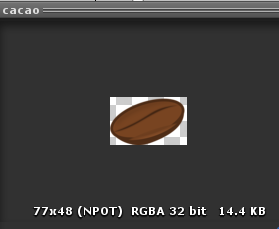
\includegraphics[width=5cm]{03TrabajoRealizado/DocProduccionR/imagenes/n3/n302.png}}
	\subfigure[Imagen de enemigo fantasma rojo]{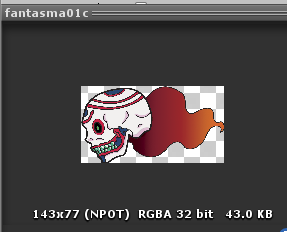
\includegraphics[width=5cm]{03TrabajoRealizado/DocProduccionR/imagenes/n3/n303.png}}
	\subfigure[Imagen de rugido de jefe enemigo]{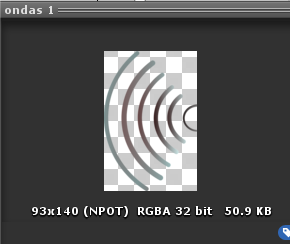
\includegraphics[width=5cm]{03TrabajoRealizado/DocProduccionR/imagenes/n3/n304.png}}
	\subfigure[Imagen de roca utilizada para daño]{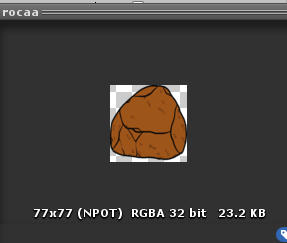
\includegraphics[width=5cm]{03TrabajoRealizado/DocProduccionR/imagenes/n3/n305.png}}
	\subfigure[Imagen de jefe enemigo jaguar Tepeyóllotl]{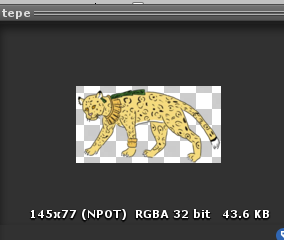
\includegraphics[width=5cm]{03TrabajoRealizado/DocProduccionR/imagenes/n3/n306.png}}
	\subfigure[Imagen de indicador de cambio de escena]{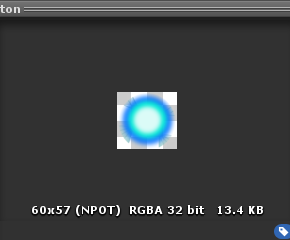
\includegraphics[width=5cm]{03TrabajoRealizado/DocProduccionR/imagenes/n3/n307.png}}
	\subfigure[Imagen de cara de jefe enemigo jaguar como indicador]{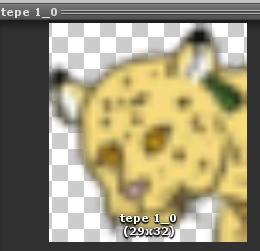
\includegraphics[width=5cm]{03TrabajoRealizado/DocProduccionR/imagenes/n3/n308.png}}
	\subfigure[Imagen de flor de vainilla para recuperar tonalli]{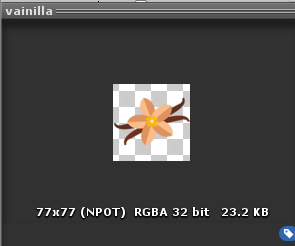
\includegraphics[width=5cm]{03TrabajoRealizado/DocProduccionR/imagenes/n3/n309.png}}
	\subfigure[Imagen de enemigo armadillo]{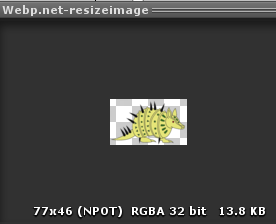
\includegraphics[width=5cm]{03TrabajoRealizado/DocProduccionR/imagenes/n3/n310.png}}
	\subfigure[Imagen de terreno rocoso]{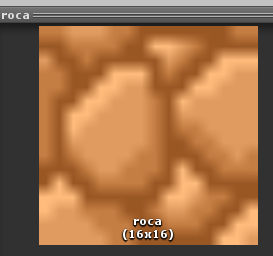
\includegraphics[width=5cm]{03TrabajoRealizado/DocProduccionR/imagenes/n3/n311.png}}
	\subfigure[Imagen de terreno con pasto]{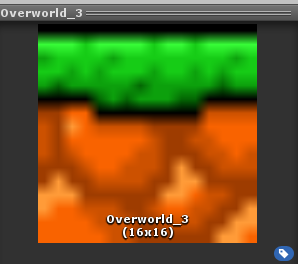
\includegraphics[width=5cm]{03TrabajoRealizado/DocProduccionR/imagenes/n3/n312.png}}
	\subfigure[Imagen de roca gigante]{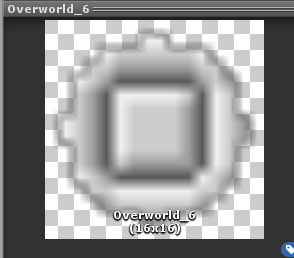
\includegraphics[width=5cm]{03TrabajoRealizado/DocProduccionR/imagenes/n3/n313.png}}
	\caption{Imágenes utilizadas para el nivel} \label{fig:n02}
\end{figure}

Después de reunir los componentes se da a la tarea de dar las acciones que realizarían descritas dentro de la figura \ref{fig:n03}. Se omite en esta parte los fantasmas enemigos que ya han sido realizados en niveles anteriores.
\begin{figure}[htbp]
	\centering
	\subfigure[Establecer que los picos tengan detección por debajo de ellos y despues caer para realizar daño.]{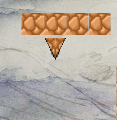
\includegraphics[width=5cm]{03TrabajoRealizado/DocProduccionR/imagenes/n3/lo0.png}}
	\subfigure[Establecer que la roca gigante detecte en una zona establecida el pase del jugador y después caiga rodando para estorbar el paso.]{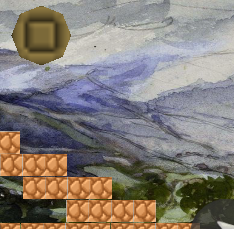
\includegraphics[width=5cm]{03TrabajoRealizado/DocProduccionR/imagenes/n3/lo1.png}}
	\subfigure[Ejemplo muestra de las plataformas que se mueven en dirección horizontal, la del lado izquierdo y vertical, la del lado derecho.]{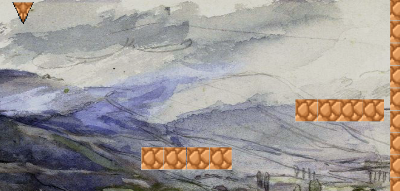
\includegraphics[width=5cm]{03TrabajoRealizado/DocProduccionR/imagenes/n3/lo2.png}}
	\subfigure[Piso que al tener contacto con el jugador este toma otra posición más abajo.]{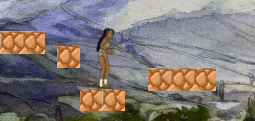
\includegraphics[width=5cm]{03TrabajoRealizado/DocProduccionR/imagenes/n3/lo3.png}}
	\subfigure[Ejemplo de como una vez que el jugador se quita de la posición sobre el piso, este vuelve a su lugar.]{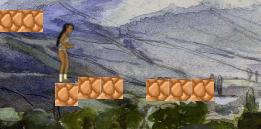
\includegraphics[width=5cm]{03TrabajoRealizado/DocProduccionR/imagenes/n3/lo4.png}}
	\caption{Muestra de comportamiento de objetos} \label{fig:n03}
\end{figure}

Ya que se tiene los objetos con los comportamientos deseados se procede a ubicarlos según correspondan como se ve en la \ref{fig:n04}.
\begin{figure}
	\centering
	\caption{Maquetado llevado al motor de juego Unity.}
	\label{fig:n04}
	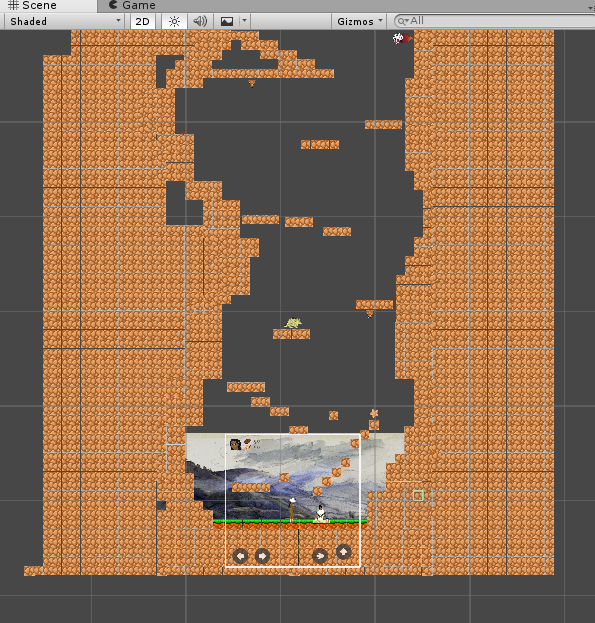
\includegraphics[width=0.5\textwidth]{03TrabajoRealizado/DocProduccionR/imagenes/n3/n301.png}
\end{figure}

Por último se establece las acciones que realiza el jefe enemigo Tepeyóllotl descritas en la siguiente figura \ref{fig:n05}.
\begin{figure}[htbp]
	\centering
	\subfigure[El enemigo se lanza en dirección al jugador con otro color.]{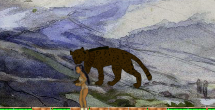
\includegraphics[width=5cm]{03TrabajoRealizado/DocProduccionR/imagenes/n3/n314.png}}
	\subfigure[El enemigo aparece rocas que van cayendo desde la parte superior.]{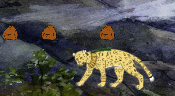
\includegraphics[width=5cm]{03TrabajoRealizado/DocProduccionR/imagenes/n3/n315.png}}
	\subfigure[El enemigo realiza un rugido.]{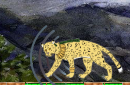
\includegraphics[width=5cm]{03TrabajoRealizado/DocProduccionR/imagenes/n3/n316.png}}
	\subfigure[El enemigo realiza un azote contra el piso apareciendo rocas a sus lados.]{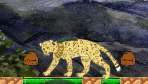
\includegraphics[width=5cm]{03TrabajoRealizado/DocProduccionR/imagenes/n3/n317.png}}
	\caption{Muestra de acciones de el jefe enemigo jaguar} \label{fig:n05}
\end{figure}
